\section{Consuntivi}
\subsubsection{Excel, individuali}

\vspace{10 mm}
\begin{spreadtab}{{tabular}{|c|c|c|c|c|c|c|c|}}
    \hline
    @\textbf{Membro} & @\textbf{Re} & @\textbf{Amm} & @\textbf{An} & @\textbf{Pg} & @\textbf{Pr} & @\textbf{Ve} & @\textbf{Totale} \\
    \hline
    @ Samuele V.   & 15          & 0          & 4         & 0          & 0     & 0     & sum(b2:f2) \\
    @ Michele Z.   & 0          & 4          & 15         & 0          & 0     & 0     & sum(b3:f3) \\
    @ Leonardo B.  & 6         & 0          & 5         & 9           & 0     & 0     & sum(b4:f4) \\
    @ Riccardo Z.  & 0          & 0          & 9          & 18          & 0     & 0     & sum(b5:f5) \\
    @ Filippo T.   & 6          & 0          & 0          & 0          & 0     & 4     & sum(b6:f6) \\
    @ Davide B.    & 0          & 3          & 3       & 0          & 0     & 3     & sum(b7:f7) \\
    \hline
    @\textbf{Ore totali} & sum(b2:b7) & sum(c2:c7) & sum(d2:d7) & sum(e2:e7) & sum(f2:f7) & sum(g2:g7) &  sum(b8:g8)\\
    \hline
    @\textbf{Costo totale} & 30*b8 & 20*c8 & 25*d8 & 15*e8 & 25*f8 & 15*g8 & sum(b9:g9)\\
    \hline
\end{spreadtab}
\vspace{10 mm}

Pg = programmatore, Pr = progettista\\

\subsubsection{Excel, produttive}

\vspace{10 mm}
\begin{spreadtab}{{tabular}{|c|c|c|c|c|c|c|c|}}
    \hline
    @\textbf{Membro} & @\textbf{Re} & @\textbf{Amm} & @\textbf{An} & @\textbf{Pg} & @\textbf{Pr} & @\textbf{Ve} & @\textbf{Totale} \\
    \hline
    @ Samuele V.   & 3          & 0          & 1         & 0          & 0     & 0     & sum(b2:f2) \\
    @ Michele Z.   & 0          & 1          & 2         & 0          & 0     & 0     & sum(b3:f3) \\
    @ Leonardo B.  & 2         & 0          & 2         & 1          & 0     & 0     & sum(b4:f4) \\
    @ Riccardo Z.  & 0          & 0          & 3          & 3          & 0     & 0     & sum(b5:f5) \\
    @ Filippo T.   & 6          & 0          & 0          & 0          & 0     & 4     & sum(b6:f6) \\
    @ Davide B.    & 0          & 3          & 2       & 0          & 0     & 3     & sum(b7:f7) \\
    \hline
    @\textbf{Ore totali} & sum(b2:b7) & sum(c2:c7) & sum(d2:d7) & sum(e2:e7) & sum(f2:f7) & sum(g2:g7) &  sum(b8:g8)\\
    \hline
    @\textbf{Costo totale} & 30*b8 & 20*c8 & 25*d8 & 15*e8 & 25*f8 & 15*g8 & sum(b9:g9)\\
    \hline
\end{spreadtab}
\vspace{10 mm}

Pg = programmatore, Pr = progettista\\

\subsubsection{Jira, produttive}
\vspace{10 mm}
\begin{spreadtab}{{tabular}{|c|c|c|c|c|c|c|c|}}
    \hline
    @\textbf{Membro} & @\textbf{Re} & @\textbf{Amm} & @\textbf{An} & @\textbf{Pg} & @\textbf{Pr} & @\textbf{Ve} & @\textbf{Totale} \\
    \hline
    @ Samuele V.   & 0          & 0          & 6        & 0          & 0     & 0     & sum(b2:g2) \\
    @ Michele Z.   & 0          & 1          & 0         & 0          & 0     & 0     & sum(b3:g3) \\
    @ Leonardo B.  & 3         & 10          & 0         & 0          & 0     & 0     & sum(b4:g4) \\
    @ Riccardo Z.  & 0          & 0          & 8          & 4          & 0     & 0     & sum(b5:g5) \\
    @ Filippo T.   & 0          & 0          & 0          & 0          & 0     & 4     & sum(b6:g6) \\
    @ Davide B.    & 0          & 0          & 11       & 0          & 0     & 1     & sum(b7:g7) \\
    \hline
    @\textbf{Ore totali} & sum(b2:b7) & sum(c2:c7) & sum(d2:d7) & sum(e2:e7) & sum(f2:f7) & sum(g2:g7) &  sum(b8:g8)\\
    \hline
    @\textbf{Costo totale} & 30*b8 & 20*c8 & 25*d8 & 15*e8 & 25*f8 & 15*g8 & sum(b9:g9)\\
    \hline
\end{spreadtab}
\vspace{10 mm}

Pg = programmatore, Pr = progettista\\
\begin{comment}
\subsection{Consuntivo RTB}

\newcommand{\totOre}{84}
\newcommand{\totCosto}{1895}

\subsubsection{Ripartizione ruoli per ore}
\begin{figure}[h]
    \centering
    \edef\percentA{\fpeval{(14/\totOre)*100}}
    \edef\percentB{\fpeval{(15/\totOre)*100}}
    \edef\percentC{\fpeval{(35/\totOre)*100}}
    \edef\percentD{\fpeval{(8/\totOre)*100}}
    \edef\percentE{\fpeval{(12/\totOre)*100}}
    \begin{tikzpicture}
        \pie[text=legend, sum=auto, radius=1.5, color={blue, red, green, orange, yellow}, hide number]
            {\percentA/Responsabile (\pgfmathprintnumber{\percentA}\%), \percentB/Amministratore (\pgfmathprintnumber{\percentB}\%), \percentC/Analista (\pgfmathprintnumber{\percentC}\%), \percentD/Programmatore (\pgfmathprintnumber{\percentD}\%), \percentE/Verificatore (\pgfmathprintnumber{\percentE}\%)}
    \end{tikzpicture}
    \caption{Distribuzione delle ore}
\end{figure}

\subsubsection{Ripartizione ruoli per costo}
\begin{figure}[h]
    \centering
    \edef\percentA{\fpeval{(420/\totCosto)*100}}
    \edef\percentB{\fpeval{(300/\totCosto)*100}}
    \edef\percentC{\fpeval{(875/\totCosto)*100}}
    \edef\percentD{\fpeval{(120/\totCosto)*100}}
    \edef\percentE{\fpeval{(180/\totCosto)*100}}
    \begin{tikzpicture}
        \pie[text=legend, sum=auto, radius=1.5, color={blue, red, green, orange, yellow}, hide number]
            {\percentA/Responsabile (\pgfmathprintnumber{\percentA}\%), \percentB/Amministratore (\pgfmathprintnumber{\percentB}\%), \percentC/Analista (\pgfmathprintnumber{\percentC}\%), \percentD/Programmatore (\pgfmathprintnumber{\percentD}\%), \percentE/Verificatore (\pgfmathprintnumber{\percentE}\%)}
    \end{tikzpicture}
    \caption{Distribuzione dei costi}
\end{figure}
\subsubsection{Ruoli per persona}

\begin{tikzpicture}
    \begin{axis}[
        ybar stacked,
        bar width=0.5cm,
        ylabel={Ore},
        xtick=data,
        xticklabels={\hspace{0.5cm}\scriptsize Samuele V.,\hspace{0.5cm}\scriptsize Michele Z.,\hspace{0.5cm}\scriptsize Leonardo B.,\hspace{0.5cm}\scriptsize Riccardo Z.,\hspace{0.5cm}\scriptsize Filippo T.,\hspace{0.5cm}\scriptsize Davide B.,\hspace{0.5cm}\scriptsize Missing Member},
        yticklabel={\pgfmathprintnumber{\tick}},
        ymin=0,
        ymax=30,
        width=15cm,
        height=6cm,
        legend style={at={(0.5,-0.15)},
        anchor=north,legend columns=-1},
        enlarge x limits=0.2,
        ]
        \addplot coordinates {(0,3) (1,0) (2,5) (3,0) (4,6) (5,0)};
        \addplot coordinates {(0,0) (1,2) (2,10) (3,0) (4,0) (5,3)};
        \addplot coordinates {(0,7) (1,2) (2,2) (3,11) (4,0) (5,13)};
        \addplot coordinates {(0,0) (1,0) (2,1) (3,7) (4,0) (5,0)};
        \addplot coordinates {(0,0) (1,0) (2,0) (3,0) (4,8) (5,4)};
        \legend{Responsabile, Amministratore, Analista, Programmatore, Verificatore}
    \end{axis}
\end{tikzpicture}

\subsubsection{Distanza dal preventivo progetto}
\begin{figure}[h]
    \centering
    \begin{tikzpicture}
        \pgfplotsset{width=0.8\textwidth, height=6cm, symbolic x coords={Responsabile, Amministratore, Analista, Programmatore, Verificatore}, xtick=data}
        
        \begin{axis}[
            ybar stacked,
            bar width=0.5cm,
            enlarge x limits=0.2,
            legend style={at={(0.5,-0.15)}, anchor=north,legend columns=-1},
            ylabel={Ore},
            xlabel={Ruolo},
            symbolic x coords={Responsabile, Amministratore, Analista, Programmatore, Verificatore},
            xtick=data,
        ]
            \addplot coordinates {(Responsabile, 12) (Amministratore, 18) (Analista, 35) (Programmatore, 22) (Verificatore, 14)};
            \addplot coordinates {(Responsabile, 10) (Amministratore, 20) (Analista, 30) (Programmatore, 25) (Verificatore, 15)};
            \legend{Attese, Effettive}
        \end{axis}
    \end{tikzpicture}
    \caption{Confronto ore attese ed effettive per ruolo}
\end{figure}

\begin{figure}[h]
	\centering
	\begin{tikzpicture}
		\pgfplotsset{width=0.8\textwidth, height=8cm, symbolic y coords={Responsabile, Amministratore, Analista, Programmatore, Verificatore}, ytick=data}
		
		\begin{axis}[
			xbar,
			bar width=0.4cm,
			enlarge y limits=0.1,
			legend style={at={(0.5,-0.15)}, anchor=north,legend columns=-1},
			xlabel={Ore},
			ylabel={Ruolo},
			symbolic y coords={Responsabile, Amministratore, Analista, Programmatore, Verificatore},
			ytick=data,
			yticklabels={Responsabile, Amministratore, Analista, Programmatore, Verificatore},
			ymajorgrids=true,
			xtick={0,20,40,60,80,100,120,140,160},
			xmajorgrids=true,
			grid style=dashed,
			ytick distance=1,
			xlabel style={yshift=10pt}, % Aggiungi un offset verticale di 10pt all'etichetta x
		]
			\addplot coordinates {(54,Responsabile) (48,Amministratore) (72,Analista) (156,Programmatore) (14,Verificatore)};
			\addplot coordinates {(14,Responsabile) (0,Amministratore) (35,Analista) (0,Programmatore) (0,Verificatore)};
			\legend{Attese, Effettive}
		\end{axis}
	\end{tikzpicture}
	\caption{Confronto ore attese ed effettive per ruolo}
\end{figure}




\begin{figure}
	\centering
	\begin{tikzpicture}
		\begin{axis}[
				ybar,
				symbolic x coords={Samuele V., Michele Z., Leonardo B., Riccardo Z., Filippo T., Davide B.},
				xtick=data,
				ylabel={Ore rimanenti},
				legend style={at={(0.5,-0.15)},
						anchor=north,legend columns=-1},
				width=0.9\textwidth,
			]
			\addplot coordinates {(Samuele V., 20) (Michele Z., 25) (Leonardo B., 15) (Riccardo Z., 30) (Filippo T., 0) (Davide B., 0) (Missing Member, 0)};
			\addplot coordinates {(Samuele V., 15) (Michele Z., 10) (Leonardo B., 20) (Riccardo Z., 25) (Filippo T., 0) (Davide B., 0) (Missing Member, 0)};
			\addplot coordinates {(Samuele V., 10) (Michele Z., 15) (Leonardo B., 10) (Riccardo Z., 20) (Filippo T., 0) (Davide B., 0) (Missing Member, 0)};
			\legend{Responsabile, Amministratore, Altri ruoli}
		\end{axis}
	\end{tikzpicture}
	\caption{Ore rimanenti per ruolo per ogni membro del gruppo}
\end{figure}
\end{comment}